	\subsection{Taxonomy of Virtualization Technologies by \textit{Chiueh}}

	\begin{figure}[!hbtp]
		\centering
		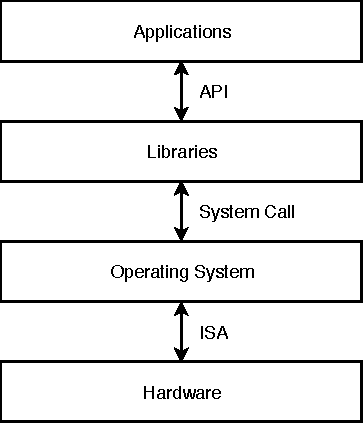
\includegraphics[width=4cm]{images/Chiueh2005.pdf}
		\vspace{-0.2cm}
		\caption{Levels of abstraction and virtualization application opportunities.\footnotemark[3]{}}
		\label{fig:VirtualizationOpportunities}
	\end{figure}
	
	\footnotetext[3]{Based on Figure 1 from the study \textit{A Survey on Virtualization Technologies} by Susanta Nanda Tzi-cker Chiueh, in 2005.}
	
	In the study, \textit{A Survery on Virtualization Technology} by \textit{Chiueh} in 2005 \cite{Chiueh2005}, a scheme is presented that's objective was to classify virtualization technologies according to the level of abstraction where they apply, see Figure \ref{fig:VirtualizationOpportunities}. Five levels are shown which correspond to \textit{Instruction Set Architecture Level}, \textit{Hardware Abstraction Layer}, \textit{Operating System Level}, \textit{Library Level} and \textit{Programming Language Level}. These levels of abstraction are described below.
	
	\subsubsection{Instruction Set Architecture Level} 
	
	This level includes the technologies relating to emulating the instruction set of the architecture in such a way that it is possible to provide a set of instructions different to the underlying hardware. This emulation implies the interpretation of the physical instructions through software. Examples of this type of technology are Bochs \cite{Bochs2018}, QEMU \cite {QEMU2018} and BIRD \cite {Nanda2006}.
	
	\subsubsection{Hardware Abstration Layer}
	
	This levels' virtualization technologies are based on abstractions that are between a real machine and an emulator. Here, the VM is an environment created and managed by a VMM, which in turn can manage VMs, in which it is possible to perform independent installations of operating systems, including their applications. These applications run as if they were executed in a real environment. Examples of these technologies are; VMware \cite{VMware2018Website}, Microsoft Virtual PC \cite{Honeycutt2003}, Denali \cite {Whitaker2002}, Xen \cite{Xen2018Website} \cite{Barham2003}, \cite{Xen2018WebsiteCambridge}, Plex86 \cite{Plex86}, Parallel \cite{Parallels2018} and UML \cite{Dike2006}, \cite{UML2006Website}. 
	
	\subsubsection{Operating System Level}
	
	This level is a virtualization tool that works through an operating system module to provide a virtualized system call interface,  such as; Jails \cite{Biederman2006} and Ensim \cite{Ensim}.
	
	\subsubsection{Library Level}
	
	At this level of abstraction, virtualization uses user-level libraries controlling the communication between the applications and the rest of the system. 
	That is to say, virtualization allows implementation as  an application binary interface (ABI) or an application programming interface (API). 
	For example, WINE \cite{Wine}, that allows supporting Windows applications on Unix-like systems. 
	Other examples are WABI \cite{WABI}, LXRun \cite{LXRUN} and Visual MainWin \cite{Fisher2006}.

	\subsubsection{Programming Language Level}
	
	This levels' virtualization technologies do not create a virtualization layer as an intermediary, but instead they implement the virtualization layer as an application that can create a virtual machine, which can be simple or complex, as is the case with the Java VM  (JVM) \cite{Lindholm1997}, Microsoft .NET common language infrastructure (CLI) \cite{Thai2003} and Parrot \cite {Parrot}. Although \textit{Chiueh} \cite{Chiueh2005} establishes an organized way to classify virtualization technologies, they do not consider the types of virtualization that exists at the same level of abstraction. In addition, it is necessary to include some technologies that have emerged in recent years.